%! TEX root = **/000-main.tex
% vim: spell spelllang=en:

%%%%%%%%%%%%%%%%%%%%%%%%%%%%%%%%%%%%%%%%%%%%%%%%%%%%%%%%%%%%%%%%%%%%%%%%%%%%%%%%
% PREAMBLE
%%%%%%%%%%%%%%%%%%%%%%%%%%%%%%%%%%%%%%%%%%%%%%%%%%%%%%%%%%%%%%%%%%%%%%%%%%%%%%%%
%! TEX root = **/000-main.tex
%%%%%%%%%%%%%%%%%%%%%%%%%%%%%%%%%%%%%%%%%%%%%%%%%%%%%%%%%%%%%%%%%%%%%%%%%%%%%%%%
%% LaTeX preamble, load in main.tex with: \input{preamble}
%%%%%%%%%%%%%%%%%%%%%%%%%%%%%%%%%%%%%%%%%%%%%%%%%%%%%%%%%%%%%%%%%%%%%%%%%%%%%%%%

\documentclass[12pt, oneside]{article}
\usepackage[a4paper, left=2.5cm, right=2.5cm, top=2.5cm, bottom=2.5cm]{geometry}

% for debugging overfulls
%\documentclass[draft, 12pt, oneside]{article}
%\usepackage[showframe, a4paper, left=2.5cm, right=2.5cm, top=2.5cm, bottom=2.5cm]{geometry}

%%%%%%%%%%%%%%%%%%%%%%%%%%%%%%%%%%%%%%%%%%%%%%%%%%%%%%%%%%%%%%%%%%%%%%%%%%%%%%%%
%% FONTS
%%%%%%%%%%%%%%%%%%%%%%%%%%%%%%%%%%%%%%%%%%%%%%%%%%%%%%%%%%%%%%%%%%%%%%%%%%%%%%%%

\usepackage[T1]{fontenc}
\usepackage{fontspec}
\usepackage{microtype}

\setmonofont[Scale=MatchLowercase]{DejaVu Sans Mono}

%%%%%%%%%%%%%%%%%%%%%%%%%%%%%%%%%%%%%%%%%%%%%%%%%%%%%%%%%%%%%%%%%%%%%%%%%%%%%%%%
%% LANGUAGE
%%%%%%%%%%%%%%%%%%%%%%%%%%%%%%%%%%%%%%%%%%%%%%%%%%%%%%%%%%%%%%%%%%%%%%%%%%%%%%%%

\usepackage{polyglossia}
\setdefaultlanguage{english}
% \setotherlanguages{spanish,catalan}

%%%%%%%%%%%%%%%%%%%%%%%%%%%%%%%%%%%%%%%%%%%%%%%%%%%%%%%%%%%%%%%%%%%%%%%%%%%%%%%%
%% BIBLIOGRAPHY
%%%%%%%%%%%%%%%%%%%%%%%%%%%%%%%%%%%%%%%%%%%%%%%%%%%%%%%%%%%%%%%%%%%%%%%%%%%%%%%%

\usepackage[
    backend=biber,
    style=numeric,
]{biblatex}
\DeclareNameAlias{default}{family-given}

\addbibresource{biblio.bib}

\usepackage{fvextra}        % Req by minted (must load before csquotes)
\usepackage{csquotes}       % For bibliography quotations
\DeclareQuoteAlias{spanish}{catalan}

%%%%%%%%%%%%%%%%%%%%%%%%%%%%%%%%%%%%%%%%%%%%%%%%%%%%%%%%%%%%%%%%%%%%%%%%%%%%%%%%
%% COMMON
%%%%%%%%%%%%%%%%%%%%%%%%%%%%%%%%%%%%%%%%%%%%%%%%%%%%%%%%%%%%%%%%%%%%%%%%%%%%%%%%

\usepackage{color, xcolor}     % more colors

\usepackage{graphicx}   % graphics
\graphicspath{{./figures/}}

\usepackage{comment}

%%%%%%%%%%%%%%%%%%%%%%%%%%%%%%%%%%%%%%%%%%%%%%%%%%%%%%%%%%%%%%%%%%%%%%%%%%%%%%%%
%% MATHS
%%%%%%%%%%%%%%%%%%%%%%%%%%%%%%%%%%%%%%%%%%%%%%%%%%%%%%%%%%%%%%%%%%%%%%%%%%%%%%%%

\usepackage{mathtools}  % amsmath + more
\usepackage{amsthm}     % Theorem enviroment
\usepackage{amssymb}    % More symbols
\usepackage{amstext}    % Text inside mathenv

%\usepackage{relsize}    % Bigger math with mathlarger{___}
%\usepackage{nicefrac}   % nice fractions in one line

%\usepackage{IEEEtrantools} % Complex equation arrays

%%%%%%%%%%%%%%%%%%%%%%%%%%%%%%%%%%%%%%%%%%%%%%%%%%%%%%%%%%%%%%%%%%%%%%%%%%%%%%%%
%% REFERENCES (load order is important)
%%%%%%%%%%%%%%%%%%%%%%%%%%%%%%%%%%%%%%%%%%%%%%%%%%%%%%%%%%%%%%%%%%%%%%%%%%%%%%%%

\usepackage{varioref} % reference far away (1)
\usepackage[colorlinks = true]{hyperref} % links in references (2)
\usepackage{cleveref} % smart references (3)
%hyperref configuration so that it doesn't contrast so much colorlinks,
\hypersetup{
   linkcolor={black},
   citecolor={black},
   %linkcolor={red!50!black},
   %citecolor={blue!50!black},
   urlcolor={blue!80!black}
}

\usepackage[bottom]{footmisc} % Footnotes at bottom of page

%%%%%%%%%%%%%%%%%%%%%%%%%%%%%%%%%%%%%%%%%%%%%%%%%%%%%%%%%%%%%%%%%%%%%%%%%%%%%%%%
%% FIGURES
%%%%%%%%%%%%%%%%%%%%%%%%%%%%%%%%%%%%%%%%%%%%%%%%%%%%%%%%%%%%%%%%%%%%%%%%%%%%%%%%

%\usepackage[export]{adjustbox}  % Adjust table size
\usepackage{float}               % Force tables and images position (H and H!)
%\usepackage{wrapfig}            % Wrap images like in HTML

\usepackage[justification=centering]{caption}
%\usepackage{subcaption}                     % Subfigures
%\usepackage[framemethod=tikz]{mdframed}     % Custom frames

%%%%%%%%%%%%%%%%%%%%%%%%%%%%%%%%%%%%%%%%%%%%%%%%%%%%%%%%%%%%%%%%%%%%%%%%%%%%%%%%
%% TABLES
%%%%%%%%%%%%%%%%%%%%%%%%%%%%%%%%%%%%%%%%%%%%%%%%%%%%%%%%%%%%%%%%%%%%%%%%%%%%%%%%

%\usepackage{colortbl, booktabs} % Better tables
%\usepackage{tabularx}
%\usepackage{longtable} % Multiple page table (does not work with tabularx)
\usepackage{xltabular, colortbl, booktabs} % longtable + tabularx (has bug with booktabs: fix below)

% Split cell in lines and more formating options inside table
\usepackage{array, multirow, multicol, makecell}

%%%
% bug fix for booktabs + xltabular incompatibility
\makeatletter
\def\@BTrule[#1]{%
  \ifx\longtable\undefined
    \let\@BTswitch\@BTnormal
  \else\ifx\hline\LT@hline
    \nobreak
    \let\@BTswitch\@BLTrule
  \else
     \let\@BTswitch\@BTnormal
  \fi\fi
  \global\@thisrulewidth=#1\relax
  \ifnum\@thisruleclass=\tw@\vskip\@aboverulesep\else
  \ifnum\@lastruleclass=\z@\vskip\@aboverulesep\else
  \ifnum\@lastruleclass=\@ne\vskip\doublerulesep\fi\fi\fi
  \@BTswitch}
\makeatother
%%%

%%%%%%%%%%%%%%%%%%%%%%%%%%%%%%%%%%%%%%%%%%%%%%%%%%%%%%%%%%%%%%%%%%%%%%%%%%%%%%%%
%% SIUNITX
%%%%%%%%%%%%%%%%%%%%%%%%%%%%%%%%%%%%%%%%%%%%%%%%%%%%%%%%%%%%%%%%%%%%%%%%%%%%%%%%

%\usepackage[alsoload=hep]{siunitx}          % SI units and uncertainties
%\sisetup{locale = FR}                       % Commas and so on for spanish
%\sisetup{separate-uncertainty=true}
%\sisetup{
  %per-mode=fraction,
  %fraction-function=\nicefrac
%}

%%%%%%%%%%%%%%%%%%%%%%%%%%%%%%%%%%%%%%%%%%%%%%%%%%%%%%%%%%%%%%%%%%%%%%%%%%%%%%%%
%% TIKZ
%%%%%%%%%%%%%%%%%%%%%%%%%%%%%%%%%%%%%%%%%%%%%%%%%%%%%%%%%%%%%%%%%%%%%%%%%%%%%%%%

%\usepackage{tikz}
%\usetikzlibrary{arrows}
%\usetikzlibrary{scopes}
%\usetikzlibrary{babel}

%%%%%%%%%%%%%%%%%%%%%%%%%%%%%%%%%%%%%%%%%%%%%%%%%%%%%%%%%%%%%%%%%%%%%%%%%%%%%%%%
%% MINTED
%%%%%%%%%%%%%%%%%%%%%%%%%%%%%%%%%%%%%%%%%%%%%%%%%%%%%%%%%%%%%%%%%%%%%%%%%%%%%%%%

\usepackage{minted}
\definecolor{codeBg}{HTML}{FFFDE7}
\setminted{
    %style=pastie,
    frame=lines,
    framesep=3mm,
    linenos,
    breaklines=true,
    encoding=utf8,
    fontsize=\footnotesize,
    bgcolor=codeBg
}

%%%%%%%%%%%%%%%%%%%%%%%%%%%%%%%%%%%%%%%%%%%%%%%%%%%%%%%%%%%%%%%%%%%%%%%%%%%%%%%%
%% CUSTOM COMMANDS
%%%%%%%%%%%%%%%%%%%%%%%%%%%%%%%%%%%%%%%%%%%%%%%%%%%%%%%%%%%%%%%%%%%%%%%%%%%%%%%%

% empty whitepage without numbering
\newcommand{\whitepage}{
    \clearpage\thispagestyle{empty}\addtocounter{page}{-1} \newpage \clearpage
}

% Add command before appendix section for page numbering: A-1
\newcommand{\appendixpagenumbering}{
    \break
    \pagenumbering{arabic}
    \renewcommand{\thepage}{\thesection-\arabic{page}}
}

%%%%%%%%%%%%%%%%%%%%%%%%%%%%%%%%%%%%%%%%%%%%%%%%%%%%%%%%%%%%%%%%%%%%%%%%%%%%%%%%
%% CUSTOM MATH OPERATORS (functions not in italic in math mode)
%%%%%%%%%%%%%%%%%%%%%%%%%%%%%%%%%%%%%%%%%%%%%%%%%%%%%%%%%%%%%%%%%%%%%%%%%%%%%%%%

%\DeclareMathOperator{\arcsec}{arcsec}
%\DeclareMathOperator{\arccot}{arccot}
%\DeclareMathOperator{\arccsc}{arccsc}
%\DeclareMathOperator{\cis}{cis}

%%%%%%%%%%%%%%%%%%%%%%%%%%%%%%%%%%%%%%%%%%%%%%%%%%%%%%%%%%%%%%%%%%%%%%%%%%%%%%%%
%% MISC
%%%%%%%%%%%%%%%%%%%%%%%%%%%%%%%%%%%%%%%%%%%%%%%%%%%%%%%%%%%%%%%%%%%%%%%%%%%%%%%%

%\usepackage{datetime} % Customize date
%% \monthyeardate\today gives the date without the day
%\newdateformat{monthyeardate}{%
    %\monthname[\THEMONTH], \THEYEAR}


%%%%%%%%%%%%%%%%%%%%%%%%%%%%%%%%%%%%%%%%%%%%%%%%%%%%%%%%%%%%%%%%%%%%%%%%%%%%%%%%
% EXTRA PACKAGES / CONFIG
%%%%%%%%%%%%%%%%%%%%%%%%%%%%%%%%%%%%%%%%%%%%%%%%%%%%%%%%%%%%%%%%%%%%%%%%%%%%%%%%

% Set default figure size
\setkeys{Gin}{width=.9\textwidth, keepaspectratio}

% Center figures by default
\makeatletter
\g@addto@macro\@floatboxreset\centering
\makeatother

% \usepackage[normalem]{ulem}
% \usepackage{dsfont}
% \usepackage{tikz}
% % \usepackage{tikzexternal}
% \usepackage{pgfplots}
% \pgfplotsset{compat=1.18}

% \usetikzlibrary{shapes,arrows,positioning,calc}

%%%%%%%%%%%%%%%%%%%%%%%%%%%%%%%%%%%%%%%%%%%%%%%%%%%%%%%%%%%%%%%%%%%%%%%%%%%%%%%%
% METADATA
%%%%%%%%%%%%%%%%%%%%%%%%%%%%%%%%%%%%%%%%%%%%%%%%%%%%%%%%%%%%%%%%%%%%%%%%%%%%%%%%

% remove when using \maketitle:
\renewcommand\and{\\[\baselineskip]}

\title{\Huge Pattern Recognition with Neural Networks\\ \Large OTDM}
\author{Aleix Boné}
\date{Fall 2022}

\begin{document}
%%%%%%%%%%%%%%%%%%%%%%%%%%%%%%%%%%%%%%%%%%%%%%%%%%%%%%%%%%%%%%%%%%%%%%%%%%%%%%%%
% TITLE
%%%%%%%%%%%%%%%%%%%%%%%%%%%%%%%%%%%%%%%%%%%%%%%%%%%%%%%%%%%%%%%%%%%%%%%%%%%%%%%%

% Default title or use titlepage.tex

%\maketitle
%! TEX root = **/000-main.tex
% vim: spell spelllang=en:

\thispagestyle{empty}
\clearpage
\setcounter{page}{-1}

\makeatletter
\begin{titlepage}
{
    \centering
    
\includegraphics[width=0.9\textwidth]{institution-logo}
    \null%
    \vspace{2em}
    {\Huge \bfseries \@title \par}
    \vspace{3em}
    {\large \scshape \@date \par}
    \vspace{2em}
    \begin{center}
    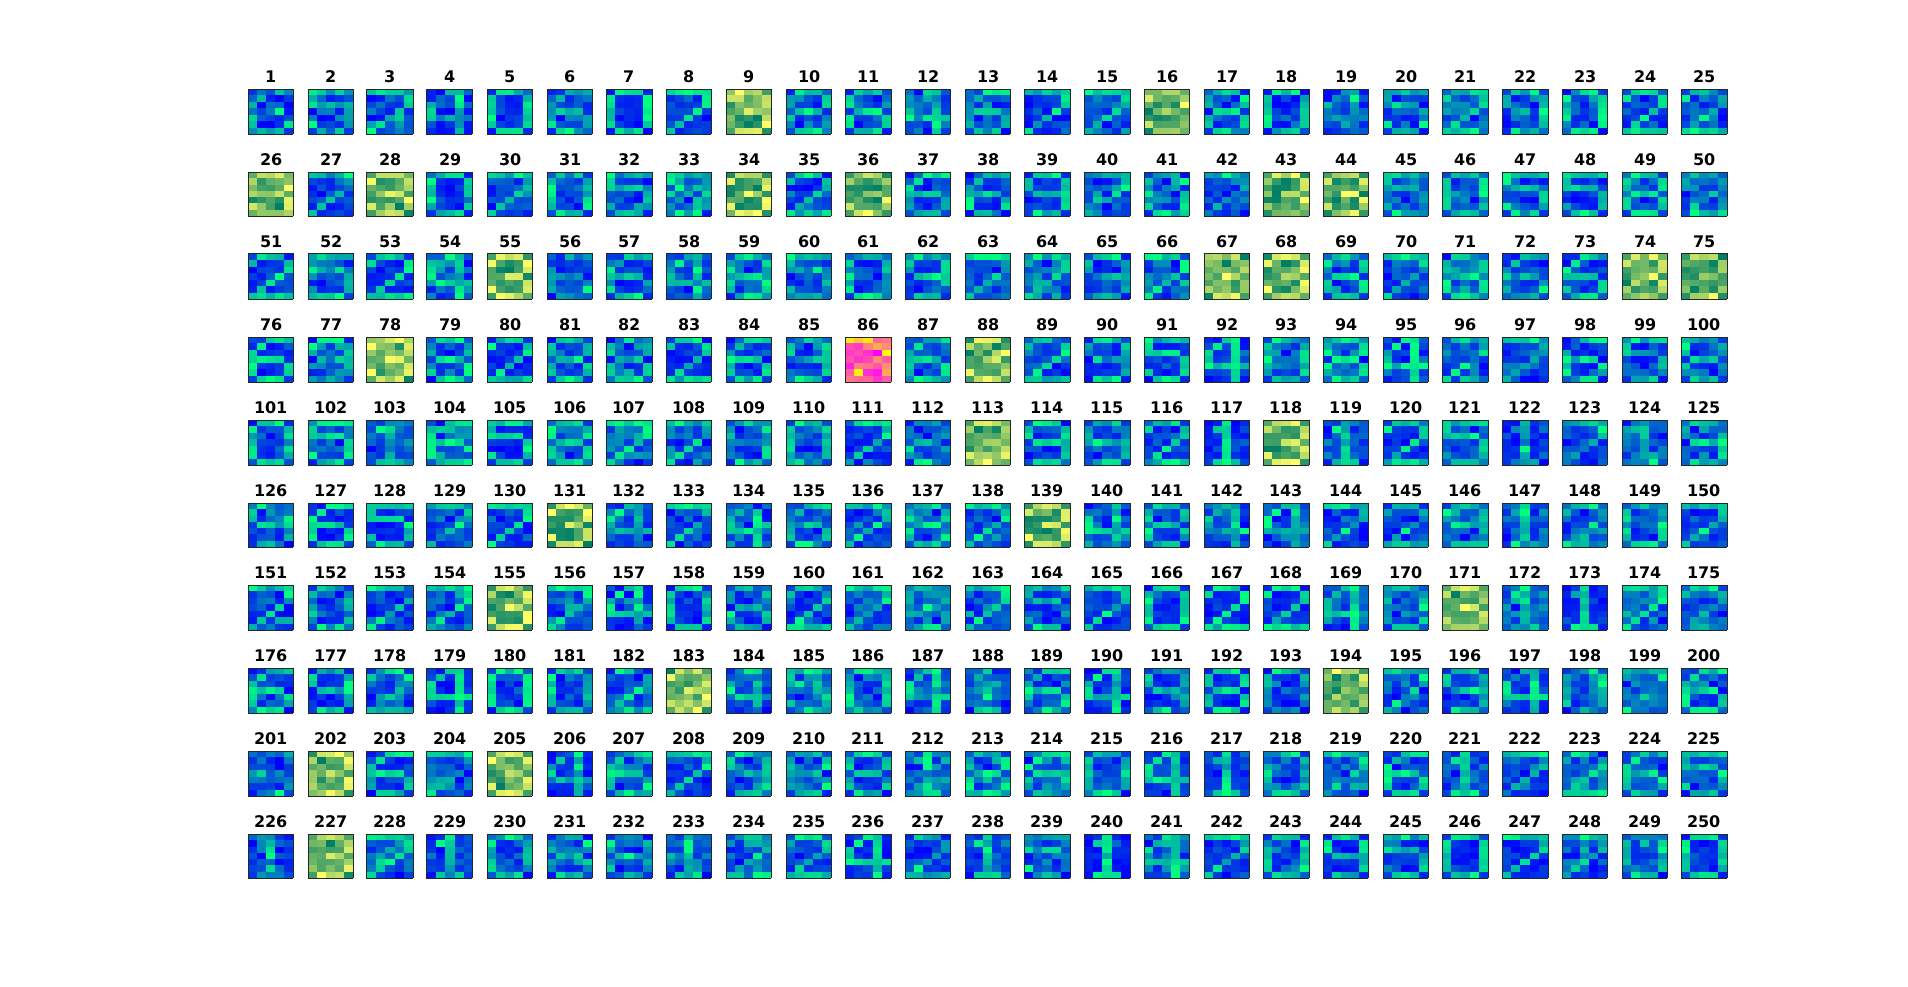
\includegraphics[width=0.9\textwidth]{../src/SGM_te_plot.png}
    \end{center}
    \vfill
\begin{center}
    % Supplementary image
\end{center}
    \vspace{1em}

    \vfill
    {{\raggedleft \large \@author \par}
    \vspace{2em}
    {\raggedleft \large \tt
        \textbf{tr\_seed:} 48089260 \\
        \textbf{te\_seed:} 26060125 \\
        \textbf{sg\_seed:} \hphantom{00}565544 \\
\par}}
}
\end{titlepage}
\makeatother


%%%%%%%%%%%%%%%%%%%%%%%%%%%%%%%%%%%%%%%%%%%%%%%%%%%%%%%%%%%%%%%%%%%%%%%%%%%%%%%%
% TOC & lists
%%%%%%%%%%%%%%%%%%%%%%%%%%%%%%%%%%%%%%%%%%%%%%%%%%%%%%%%%%%%%%%%%%%%%%%%%%%%%%%%

% \pagenumbering{Roman}

%\setcounter{tocdepth}{2}
% \tableofcontents \pagebreak

% \listoffigures \listoftables \clearpage

% \pagenumbering{arabic}

%%%%%%%%%%%%%%%%%%%%%%%%%%%%%%%%%%%%%%%%%%%%%%%%%%%%%%%%%%%%%%%%%%%%%%%%%%%%%%%%
% SECTIONS
%%%%%%%%%%%%%%%%%%%%%%%%%%%%%%%%%%%%%%%%%%%%%%%%%%%%%%%%%%%%%%%%%%%%%%%%%%%%%%%%

% Paragraph spacing (placed after ToC)
\setlength{\parskip}{1em plus 0.5em minus 0.2em}
%\setlength{\parindent}{0pt}

%! TEX root = ../000-main.tex
\section{Study of Convergence}%
\label{sec:convergence}

We'll study the global and local convergence of
the three algorithms only in terms of the objective function
$\tilde L$. In order to do so, we'll use a small dataset
to reduce the computational cost of the experiments. The
parameters to generate the dataset are the following:
\begin{center}
    \begin{BVerbatim}
    tr_p = 250; te_q = 250; tr_freq = 0.5;
    \end{BVerbatim}
\end{center}

We'll run the program for all combinations of target digit,
$\lambda$, and algorithm shown below:
\begin{alignat*}{3}
    \text{digit} &\in \{0, 1, 2, 3, 4, 5, 6, 7, 8, 9\} & \quad
    \lambda &\in \{0, 0.01, 0.1\} & \quad
    \text{algorithm} &\in \{\text{GM}, \text{QNM}, \text{SGM}\}
\end{alignat*}
Which amounts to $10 \cdot 3 \cdot 3 = 90$ instances to be solved. To
ensure that the results are reproducible, we'll use the following seeds:
\begin{center}
    \begin{BVerbatim}
        tr_seed=48089260; te_seed=26060125; sg_seed=565544;
    \end{BVerbatim}
\end{center}
Finally, the maximum number of iterations will be set to \texttt{kmax=1000}
(\texttt{sg\_emax} for \texttt{SGM}).



\subsection{Global convergence}

\Cref{fig:lambda_L} shows the relationship between the parameter
$\lambda$ and the value of the objective function $\tilde L$ at
the convergence of the algorithms. There is a clear positive
trend between $\lambda$ and $L^*$ for all three algorithms.

\begin{figure}[ht]
\input{../analysis/lambda_L.tikz}
\caption{Value of $L^*$ as a function of $\lambda$ for the three algorithms.}%
\label{fig:lambda_L}
\end{figure}

We can also see that $QNM$ and $GM$ behave similarly, in fact, they
converge to the same value of $L^*$ in most cases. On the other
hand, $SGM$ is consistently worse in terms of the value of $L^*$ than
the other two algorithms.

The best combination of algorithm and $\lambda$ is $GM$ (Gradient method)
with $\lambda = 0$. Obtaining the best value of $L^*=10^{-5}$, as shown
in \cref{tab:lambda_L}.

% Global convergence: analyse the global convergence of every algorithm and how
% this global convergence property depends on the value of the regularization parameter
% ������������. Which combination algorithm-������������ gives the best results in terms of global converge? In
% particular, discuss the application to the SGM of the conditions for global convergence.

\begin{table}[ht]
    \caption{Average value of $L^*$ with standard deviation $\sigma$ for each algorithm and $\lambda$}%
    \label{tab:lambda_L}%
    \begin{tabular}{cS[table-format=1.2]S[table-format=1.5(2)]}
	\toprule
    Algorithm & $\lambda$ & {$L^* \pm \sigma$}  \\ \midrule
	GM        & 0         & 0.00001(2)                   \\
	QNM       & 0         & 0.0008(17)                 \\
	SGM       & 0         & 0.0018(3)                  \\
	\addlinespace
	GM        & 0.01      & 0.05(2)                   \\
	QNM       & 0.01      & 0.05(2)                   \\
	SGM       & 0.01      & 0.07(3)                   \\
	\addlinespace
	GM        & 0.1       & 0.13(3)   \\
	QNM       & 0.1       & 0.13(3)   \\
	SGM       & 0.1       & 0.29(13)                   \\ \bottomrule
\end{tabular}

\end{table}

% \begin{figure}[ht]
% \input{../analysis/iter_alg.tikz}
% \caption{Number of iterations for each algorithm}%
% \label{fig:iter_alg}
% \end{figure}

\pagebreak
\subsection{Local convergence}

\subsubsection{Speed of convergence}

% Compare the speed of convergence of the three algorithms in terms of the
% execution time and number of iterations.

\Cref{fig:lambda_iter} shows the number of iterations for each
combination of algorithm and $\lambda$ for the different target
numbers. The iterations are in logarithmic scale and we show
the maximum number of iterations for each algorithm as a red line
(1000 for $GM$ and $QNM$ and 125125 for $SGM$).

\begin{figure}[H]
\input{../analysis/lambda_iter.tikz}
\caption{Number of iterations for each algorithm}%
\label{fig:lambda_iter}
\end{figure}

The first thing we observe is that a bigger $\lambda$ reduces
the number of iterations. This is expected since the regularization
parameter $\lambda$ is a trade-off between the data fitting and
the smoothness of the solution. The exception are some cases in
$QNM$ where we seem to converge in less than 10 iterations.

The iterations for $QNM$ and $GM$
are in the same order of magnitude but we can see some
notable differences. For instance, $GM$ takes more iterations
in most cases. Also, for $\lambda = 0$ and target number 8,
$GM$ takes reaches the maximum number of iterations (1000), while
$QNM$ converges in less than 100 iterations in all but two cases.

Another interesting observation is that the differences between
iterations between digits are more consistent in $QNM$, with much
less variability. The exception is when $\lambda = 0$, where
$QNM$ takes either less iterations than with the regularizer or
more iterations.

For $SGM$, we cannot compare the number of iterations with the
other two algorithms, but we can see that with $\lambda = 0$,
$SGM$ does not converge in 5 instances, while it converges in
the rest.

If we now look at the execution time for each algorithm and
how it depends on $\lambda$ as shown in \cref{fig:lambda_tex_niter},
where we show the execution time on the left subplot and the
number of iterations on the right subplot. We can see that
when $\lambda = 0$, there is a wide range of execution times
across all algorithms, but the fastest algorithm is $QNM$.

When using a regularizer, the execution time is more consistent
and the fastest algorithm is $SGM$ by a noticeable margin.
This is despite the fact that $SGM$ has more iterations than the
other two methods, but as we will see, the execution time per
iteration is much lower for $SGM$, since the computations are
much simpler.

\begin{figure}[H]
\input{../analysis/lambda_tex_niter.tikz}
\caption{Number of iterations for each algorithm}%
\label{fig:lambda_tex_niter}
\end{figure}

% Analyse how the speed of convergence of the three algorithms depend on the
% value of lambda and try to find an explanation for the observed dependence,
% if any.

% Analyze the running time per iteration and try to find an explanation for
% the different values among the three algorithms.

\subsubsection{Execution time per iteration}

Let us now look at the execution time per iteration for each
algorithm and how it depends on $\lambda$. Since the execution time
of $SGM$ is much lower than the other two, we cannot plot it in the
same scale. In \cref{fig:lambda_tex_over_niter_comb} we show the
boxplots of the execution time per iteration for each algorithm
and $\lambda$, notice that for $GM$ and $QNM$ we use
\si{\milli\second} (\SI{1e-3}{\second}) as the unit of time, while for $SGM$ we use
\si{\micro\second} (\SI{1e-6}{\second}).

The fastest execution time per iteration is for $SGM$, with a mean
of \SI{13}{\micro\second} per iteration. It seems that the effect
of the regularizer is negligible for $SGM$, with no noticeable change
between the different values of $\lambda$.

For $GM$ and $QNM$, we see a clear effect of the regularizer on
the execution time per iteration. What's interesting is that
not only is there a noticeable difference between not having
a regularizer and having one, but also between
different values of $\lambda$. This may be caused by the fact that
not all the time we measure is part of the actual iterations of the
algorithm, but it also includes the initialization of the algorithm,
memory allocation, etc. This means that with higher values of $\lambda$,
when the algorithm converges faster the execution time per iteration
is higher since the initialization time is a bigger part of the total.

\begin{figure}[H]
    \input{../analysis/lambda_tex_over_niter_comb.tikz}
    \caption{Execution time per iteration as a function of $\lambda$ for the three algorithms.}%
    \label{fig:lambda_tex_over_niter_comb}
\end{figure}

\subsection{Discussion}

Our objective was to answer the question of which combination of algorithm and $\lambda$
is the most efficient, we have seen that the global convergence of
$GM$ and $QNM$ is better than $SGM$ for all values of $\lambda$
(\cref{fig:lambda_L,tab:lambda_L}). However,
the execution time of $SGM$ is much lower than the other two
(\cref{fig:lambda_tex_niter,fig:lambda_tex_over_niter_comb}).

Given all that, we have to consider whether the additional computation
time of $GM$ and $QNM$ is worth the improvement in global convergence.
The answer to this question depends on the application, but we argue that
by what we have seen in our problem of $SLNN$: $SGM$ with $\lambda=0.01$ is the best choice;
it is much faster and gives similar results to the other two algorithms.
We could also use $\lambda=0.1$, but probably not $\lambda=0$, since
we have seen that it reached the maximum number of iterations in some cases.

%! TEX root = ../000-main.tex

\section[Study of Accuracy]{Study of Accuracy for large problems}

\subsection{Experiment setup}

We'll study the accuracy of the three algorithms. To do so, we
repeat the experiments of \cref{sub:convergence_setup} but this time
we'll use a more realistic dataset, generated from the following
parameters:
\begin{center}
    \begin{BVerbatim}
    tr_p = 20000; te_q = tr_p/10; tr_freq = 0.0;
    \end{BVerbatim}
\end{center}

The main differences are that now, we have a much larger training and test
sets and that the training set is now balanced, meaning that it has the same
number of samples from each class.

We'll use the values of $\lambda$ that gave the best accuracy in
the experiments from~\cref{sec:convergence} for each algorithm.
These previous results are shown in~\cref{tab:te_acc_250}.

\begin{table}[ht]
    \caption{Accuracy on test set from previous experiment (\texttt{tr\_p = 250}) with
    the highest average accuracy for each method in bold}%
    \label{tab:te_acc_250}%
    \begin{talltblr}{
	colspec={cS[table-format=1.2]S[table-format=2.1(1)]}
	}
	\toprule
	Algorithm & {{{$\lambda$}}} & {{{$Accuracy^{TE}\pm \sigma$}}} \\ \midrule
	GM        & 0               & 99.2(9)                         \\
	QNM       & 0               & 99.4(7)                         \\
	\SetRow{bg=gray9,font=\bfseries}
	SGM       & 0               & 99.6(5)                         \\
	\addlinespace
	\SetRow{bg=gray9,font=\bfseries}
	GM        & 0.01            & 99.5(8)                         \\
	\SetRow{bg=gray9,font=\bfseries}
	QNM       & 0.01            & 99.5(8)                         \\
	SGM       & 0.01            & 99.4(5)                         \\
	\addlinespace
	GM        & 0.1             & 97(5)                           \\
	QNM       & 0.1             & 97(5)                           \\
	SGM       & 0.1             & 94(4)                           \\ \bottomrule
\end{talltblr}

\end{table}

\pagebreak
% \subsection{Results}

% For this analysis, our main focus is on the accuracy obtained on the test set and
% the time it takes to obtain it.

\subsection{Accuracy}

Let's start by looking at the accuracy obtained from the three algorithms
taking into account the different values of $\lambda$. The results are shown in
\cref{fig:lambda_acc_2}. We can see that the accuracy values obtained from the
train and test sets are very similar, which is a good sign that the model is
not overfitting. Moreover, the accuracy values for each method are very similar
to each other (except some outliers on $QNM$ with $\lambda = 0$). Which would
suggest that the three methods are equally good at finding the optimal solution
when using the same regularization parameter.

\begin{figure}[H]
    \input{../analysis/acc_lambda_acc.tikz}
    \caption{Accuracy on train and test set for all algorithms with different values of $\lambda$}
    \label{fig:lambda_acc_2}
\end{figure}

Given that the accuracy of $\lambda=0.1$ is notably lower than the rest it
makes it difficult to distinguish the differences from the other values.
Any accuracy lower than 90\% given the proportion of the samples is no better
than classifying everything as a non-match.
% Therefore, the values obtained with $\lambda=0.1$ are not considered in the following analysis.
In fact, if we look at the results for one of the instances with accuracy 89.95\%,
we can see that everything is a false negative as illustrated in \cref{fig:fneg} where
we can see that everything is classified as not a 3.

\begin{figure}[H]
    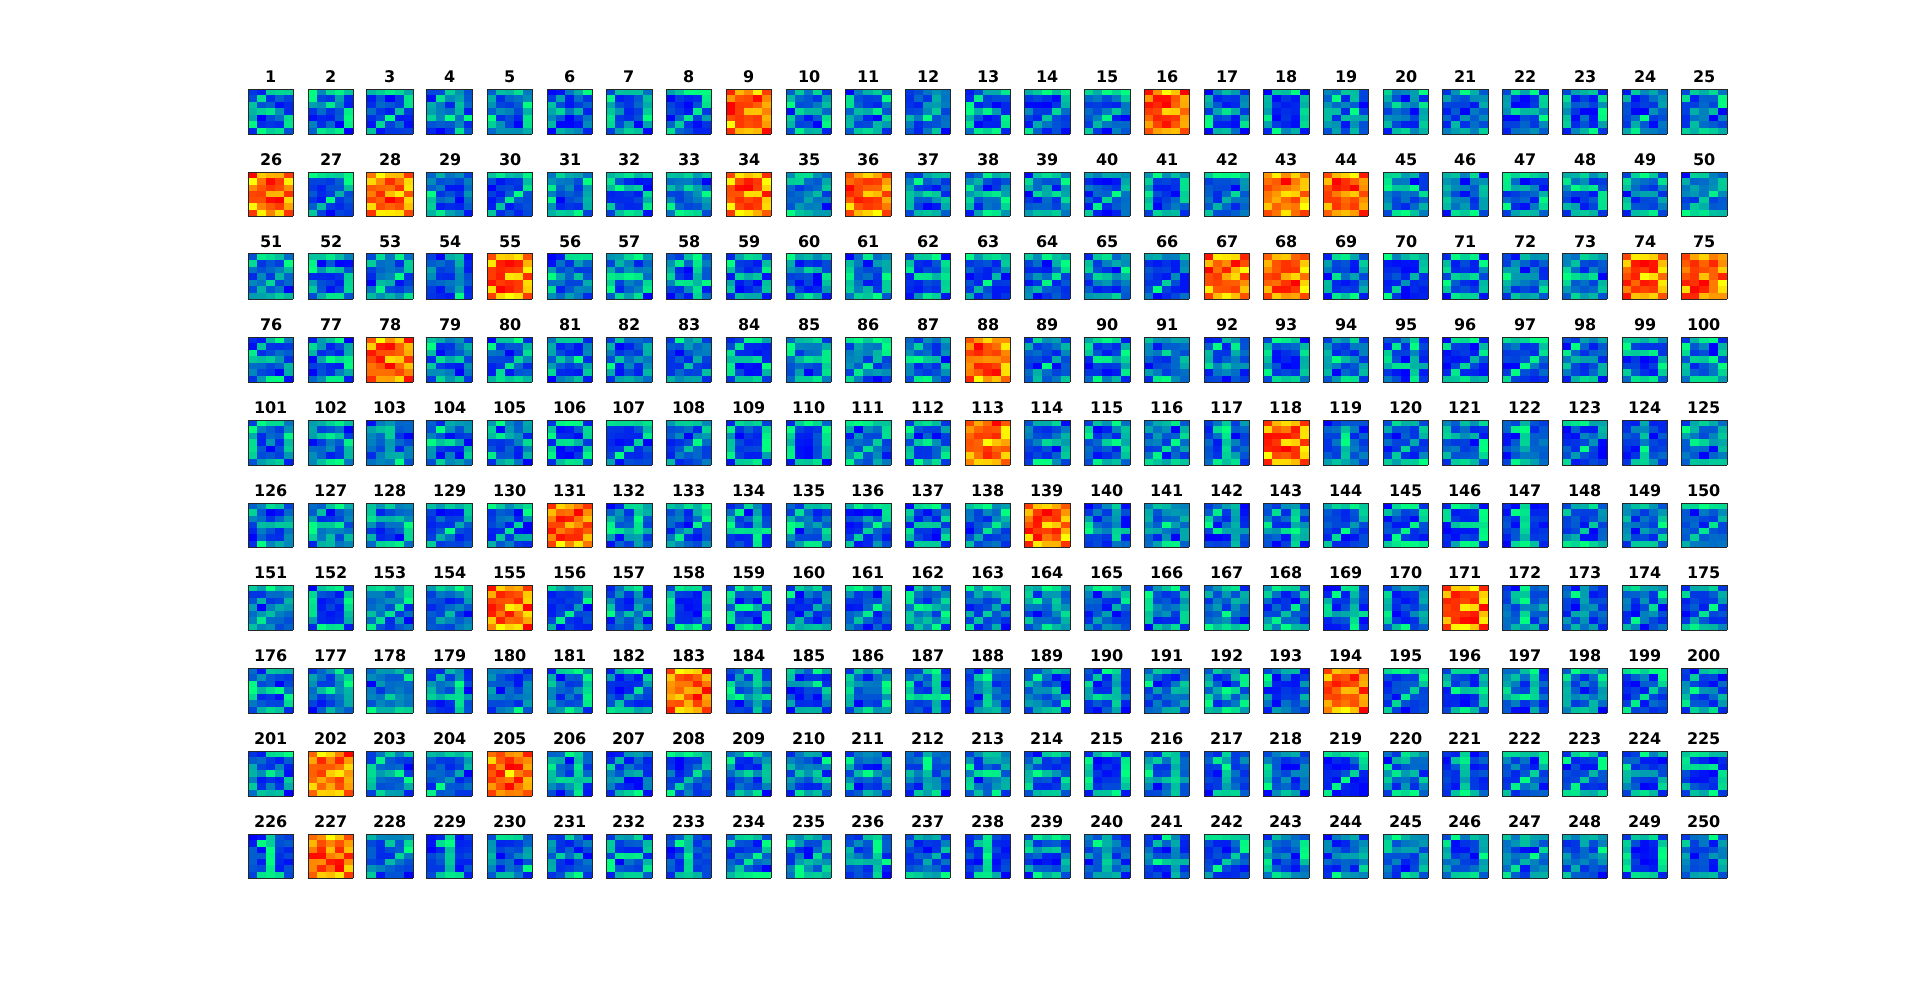
\includegraphics[width=\textwidth]{../src/SGM_te_plot_2k_01.png}
    \caption{Sample of first 250 from test set of $SGM$ with $\lambda=0.1$ and target 3,
    false negatives are shown in red and true negatives in blue}
    \label{fig:fneg}
\end{figure}

For reference, \cref{fig:fneg-001} shows the same sample but with $\lambda=0.01$, where
we can see that now there are true positives (in green) and much fewer false negatives.
The accuracy in this case is 97.95\%. There are no false positives (pink) in this particular
sample.

\begin{figure}[H]
    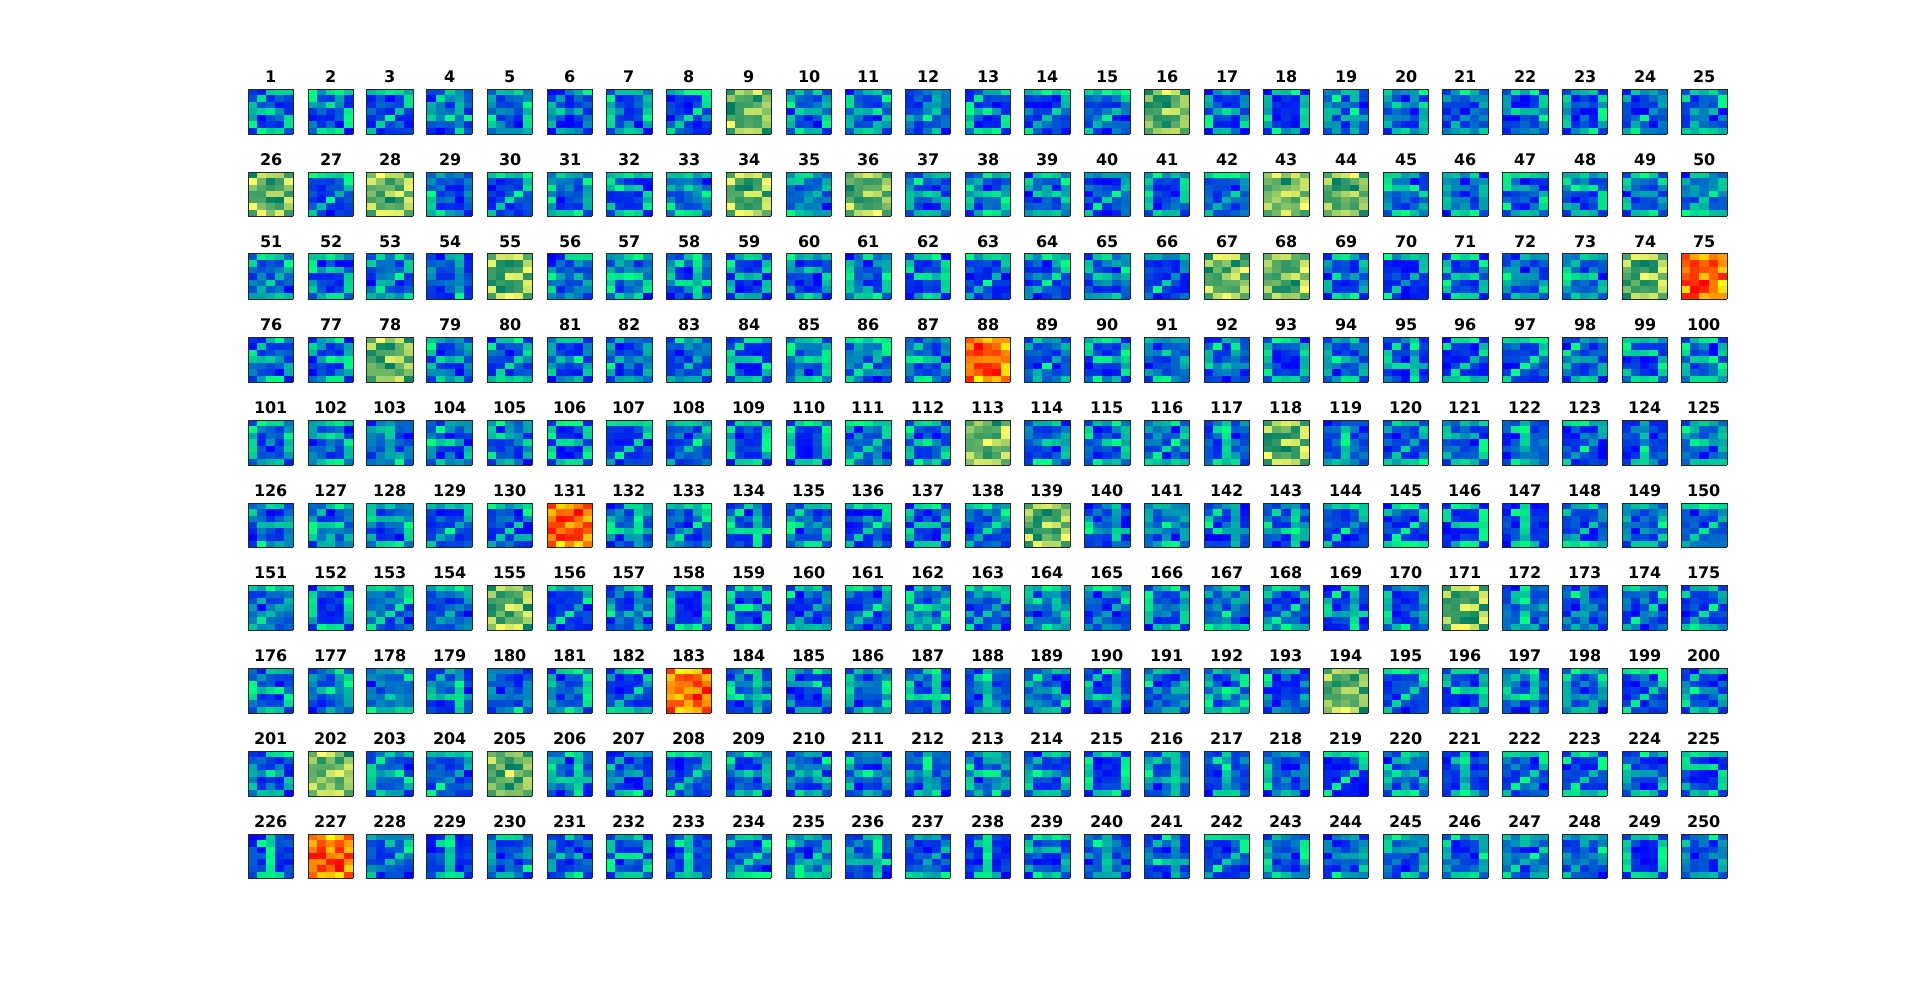
\includegraphics[width=\textwidth]{../src/SGM_te_plot_2k_001.png}
    \caption{Sample of first 250 from test set of $SGM$ with $\lambda=0.01$ and target 3,
    false negatives are shown in red, true negatives in blue and true positives in green}
    \label{fig:fneg-001}
\end{figure}

\pagebreak
Let's now look at the detail on the accuracy of the \emph{test} set for
$\lambda \neq 0.1$. This detailed magnification is shown in~\cref{fig:lambda_acc_2_detail}.
There, we can see that without regularization ($\lambda = 0$) the accuracy is
near 99.7\% for all three methods, while with $\lambda = 0.01$ the accuracy is slightly
lower, but still very high. Keep in mind that for $QNM$ we are omitting 2 outliers on
$\lambda = 0$ that are not shown in the figure. $SGM$ has slightly higher accuracy in
both cases.

\begin{figure}[H]
    \input{../analysis/acc_te_detail.tikz}
    \caption{Detail on the accuracy on test set for all algorithms for values of $\lambda \neq 0.1$ and
    omitting outliers}
    \label{fig:lambda_acc_2_detail}
\end{figure}

From \cref{fig:lambda_acc_2,fig:lambda_acc_2_detail} we can draw the following conclusions regarding
the accuracy of the three algorithms and the different values of $\lambda$:
\begin{enumerate}
    \item They all have very similar accuracy, however $SGM$ outperforms the other by a
        small margin.
    \item Without regularization we obtain very high accuracies, but we risk not reaching
        a proper solution (as is the case with the outliers in $QNM$ in our results).
\end{enumerate}

Therefore, in terms of accuracy, we can conclude that $SGM$ is the best method.

\pagebreak
\subsection{Training speed}

Let's now look at the training speed of the algorithms. We'll start by looking
at the time it takes to train the model for each value of $\lambda$ and
algorithm. The results are shown in~\cref{fig:lambda_time_2}. The time
is in logarithmic scale to better see the differences between the values.

From the figure, we can see that $SGM$ is the fastest method in all cases, by more
than an order of magnitude. This difference is even more noticeable when
we don't use regularization ($\lambda = 0$). In this case, $SGM$ takes
no more than 3 seconds (except for one outlier at 11), while the other
two take up to 100 seconds, and even the fastest outliers of
$QNM$ and $GM$ take more than 10 seconds.

\begin{figure}[H]
    \input{../analysis/acc_te_tex.tikz}
    \caption{Time to train the model for all algorithms with different values of $\lambda$}
    \label{fig:lambda_time_2}
\end{figure}

If we now look at the number of iterations%
\footnote{We use epochs instead of iterations for $SGM$ as explained in~\cref{ssub:epochs}.
In this case, ${e^{SG} = k^{SG}/100}$.}
instead of the execution time, we can see that the high execution times for
$QNM$ and $GM$ are due to the fact that they do not converge. Looking at
\cref{fig:lambda_nie_2} we can see that they reach
the maximum number of iterations set in the experiment (1000) in most cases
when $\lambda = 0$, to the point that the boxplot is a flat line at Iterations = 1000.
There is also an instance where $SGM$ reaches the maximum number of iterations.

\begin{figure}[H]
    \input{../analysis/acc_te_nie.tikz}
    \caption{Iterations to train the model for all algorithms with different values of $\lambda$}
    \label{fig:lambda_nie_2}
\end{figure}

From the results on execution time, there is a clear winner: $SGM$ is the fastest
method by far. Combining this with the fact that it also has the highest accuracy,
we can conclude that $SGM$ with $\lambda = 0.01$ is the algorithm and regularization
parameters from what we have tested. We cannot use $\lambda = 0$ as we have seen that
it can lead to non-convergence, which did not happen with our smaller dataset in the
first experiment but with this larger one we had one case.

\pagebreak
\subsection{Differences with previous experiment}

Now, we will compare the plots of execution time and iterations
from the first experiment (Experiment 1), with
the ones from this new one which has a bigger data size (Experiment 2). The aim of the comparison
is to quantify how the increase in size of the dataset
from 250 to $20\,000$ affects the performance of each algorithm.

\subsubsection{Iterations}

\Cref{fig:comp_niter} shows the comparison of the number
of iterations from both experiments. There are some notable differences:
\begin{enumerate}
    \item When $\lambda = 0$ in Experiment 2 we reach the maximum number of iterations
        before convergence in most cases, this is not the case in Experiment 1 where
        we have much more variability. This shows that regularization is important
        with bigger datasets.
    \item When $\lambda \neq 0$, the behaviour of both experiments is similar, with
        a slight increase in the number of iterations in Experiment 2, but not
        significant.
\end{enumerate}

\begin{figure}[H]
    \input{../analysis/comp_niter.tikz}
    \caption{Comparison of the number of iterations for the two experiments}
    \label{fig:comp_niter}
\end{figure}

\pagebreak
\subsubsection{Execution time per iteration}

\Cref{fig:comp_tex} shows the comparison of the execution time per iteration in the
two experiments. There is a clear difference in computation time between the two, but
we can see that a priori, the increase in execution time per iteration of
$SGM$ is smaller than the increase in execution time per iteration of $QNM$ and $GM$.

\begin{figure}[H]
    \input{../analysis/comp_tex.tikz}
    \caption{Comparison of the execution time per iteration for the two experiments}
    \label{fig:comp_tex}
\end{figure}

To quantify the increase in execution time per iteration, we can look at
\cref{fig:comp_ratio}. There, we can clearly see that indeed the increase
in execution time per iteration of $SGM$ is much smaller than the increase
in execution time per iteration of $QNM$ and $GM$. Keep in mind, that
the increase in data is 250 \textrightarrow{} $20\,000$, which is a factor of 80.
$GM$ and $QNM$ seem to have a linear increase in execution time per iteration,
while $SGM$ has sublinear increase.

\begin{figure}[H]
    \input{../analysis/acc_tnie_ratio.tikz}
    \caption{Comparison of the increase the execution time per iteration from one
    experiment to the other}
    \label{fig:comp_ratio}
\end{figure}

% \begin{figure}[H]
%     \input{../analysis/acc_tex_over_nie.tikz}
%     \caption{Time to train the model for all algorithms with different values of $\lambda$}
%     \label{fig:tex_over_nie2}
% \end{figure}

\subsection{Conclusions}

In the discussion of the previous experiment (\cref{ssub:discussion}) we concluded that
$SGM$ with $\lambda = 0.01$ was the best method for the minimization of
$\tilde L$. In this experiment, we have seen that again, $SGM$ with $\lambda = 0.01$
is the best method when aiming to maximize the accuracy on the test set.

The decision from the first experiment was opinionated since
$SGM$ did not give the lowest value of $\tilde L$, but it was small enough and
considerably faster than the others. In this experiment, $SGM$ outperforms the other
methods both in terms of accuracy and execution time. Not only that, but also, we have
seen that the increase in execution time per iteration of $SGM$ is much smaller than
the increase in execution time per iteration of $QNM$ and $GM$ in relation to the
increase in data size.

With our limited sample size,
we can conclude that for larger datasets,
$SGM$ is the best method to use by all accounts. We can also conclude that the value
of the regularization parameter $\lambda$ is really important and should be tuned
carefully. On one hand, if the value of $\lambda$ is too small, the algorithm can take a long time
to converge or exceed the maximum number of iterations. On the other hand, if the value
of $\lambda$ is too large, the algorithm can converge to a local minimum were all the results
are negative, which is undesirable.



% \nocite{*}

% \printbibliography

\end{document}
